\begin{figure}[htb]
	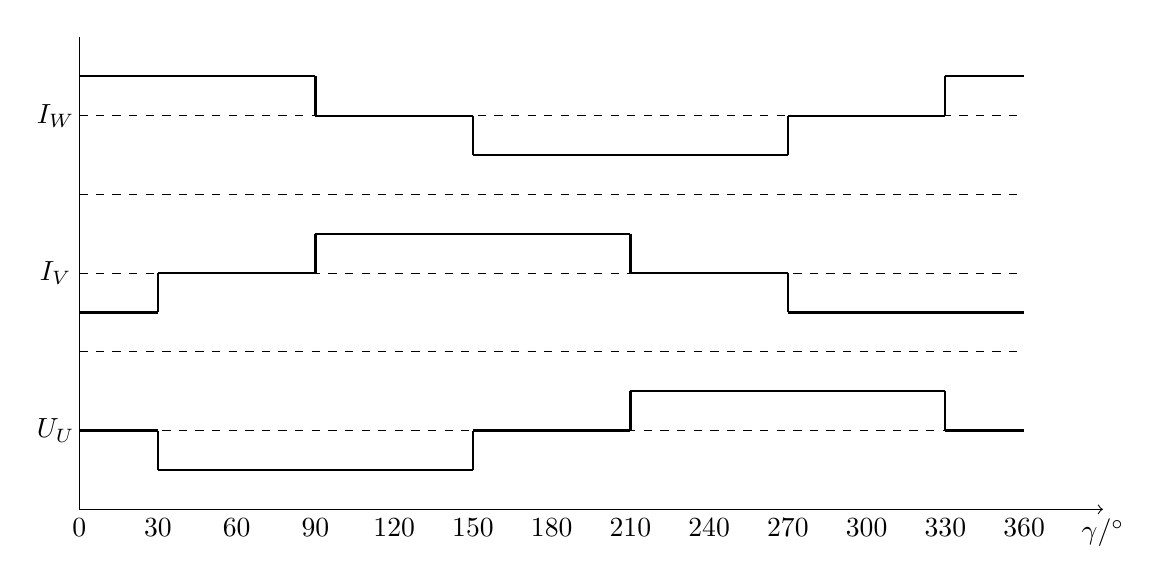
\begin{tikzpicture}
	
	% horizontal axis
	\draw[->] (0,0) -- (13,0) node[anchor=north] {$\gamma/^{\circ}$};
	\draw[dashed] (0, 1) -- (12,1);
	\draw[dashed] (0, 2) -- (12,2);
	\draw[dashed] (0, 3) -- (12,3);
	\draw[dashed] (0, 4) -- (12,4);
	\draw[dashed] (0, 5) -- (12,5);
	
	% vertical axis
	\draw (0,0) -- (0,6) node[anchor=east] {};
	
	% labels
	\draw	(0,0) node[anchor=north] {0}
	(1,0) node[anchor=north] {30}
	(2,0) node[anchor=north] {60}
	(3,0) node[anchor=north] {90}	
	(4,0) node[anchor=north] {120}
	(5,0) node[anchor=north] {150}
	(6,0) node[anchor=north] {180}
	(7,0) node[anchor=north] {210}
	(8,0) node[anchor=north] {240}
	(9,0) node[anchor=north] {270}
	(10,0) node[anchor=north] {300}
	(11,0) node[anchor=north] {330}
	(12,0) node[anchor=north] {360};	
	
	\draw (-0.3, 5) node{{$I_W$}};
	\draw (-0.3, 3) node{{$I_V$}};
	\draw (-0.3, 1) node{{$U_U$}};
	
	%draw Iw
	\draw [thick] 
	(0, 5.5)  --  (3, 5.5)
	(3, 5.5)  --  (3, 5.0)
	(3, 5.0)  --  (5, 5.0)
	(5, 5.0)  --  (5, 4.5)
	(5, 4.5)  --  (9, 4.5)
	(9, 4.5)  --  (9, 5.0)
	(9, 5.0)  -- (11, 5.0)
	(11, 5.0) -- (11, 5.5)
	(11, 5.5) -- (12, 5.5);
	
	%draw Iv
	\draw [thick] 
	(0, 2.5)  --  (1, 2.5)
	(1, 2.5)  --  (1, 3.0)
	(1, 3.0)  --  (3, 3.0)
	(3, 3.0)  --  (3, 3.5)
	(3, 3.5)  --  (7, 3.5)
	(7, 3.5)  --  (7, 3.0)
	(7, 3.0)  --  (9, 3.0)
	(9, 3.0)  --  (9, 2.5)
	(9, 2.5)  -- (12, 2.5);
	
	%draw Iu
	\draw [thick] 
	(0, 1.0)  --  (1, 1.0)
	(1, 1.0)  --  (1, 0.5)
	(1, 0.5)  --  (5, 0.5)
	(5, 0.5)  --  (5, 1.0)
	(5, 1.0)  --  (7, 1.0)
	(7, 1.0)  --  (7, 1.5)
	(7, 1.5)  -- (11, 1.5)
	(11, 1.5) -- (11, 1.0)
	(11, 1.0) -- (12, 1.0);
	
	\end{tikzpicture}
	\caption{Idealisierte Stromverl\"aufe}
	\label{dia:aufgabe2a_strom}
\end{figure}